% !TEX root = ../Documentation.tex

\section{Analysis}
\label{sec:analysis}
In this section, we analyze the previous Ampersand parser in order to understand its workings and signal the improvement points.

\subsection{System overview (R-M)}
The requirements of the new parser have been described in the project planning \citenac{plan}.
Basically, both the old and the new parser must be able to make a conversion from a text file (ADL-script) to a parse tree (the P-structure).
\autoref{fig:data-flow-1} depicts this data flow.
%
\begin{figure}[htb!]
	\centering
	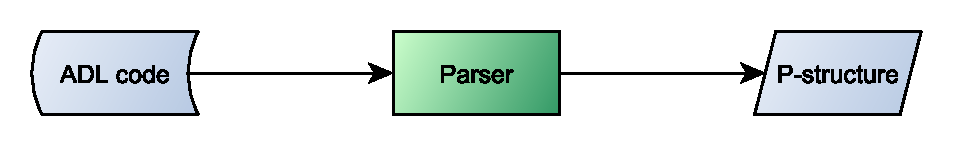
\includegraphics[width=0.586\textwidth]{Figures/DataFlow1}
	\caption{Relevant data flow for the Ampersand parsing component}
	\label{fig:data-flow-1}
\end{figure}

Often, the parsing component is separated into a lexer (that converts text to tokens) and the actual parser (that converts the tokens into the parse tree).
Since this separation is considered beneficial for both maintainability and performance \citeac{parsec}, we assumed from the beginning that the new Ampersand parser would be separated in this way.
This is depicted in \autoref{fig:data-flow-2}.
The previous parser also had a separate lexer, but the name was scanner instead.
%
\begin{figure}[htb!]
	\centering
	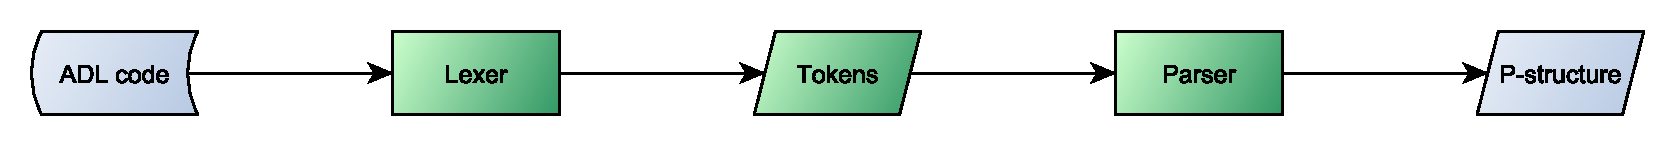
\includegraphics[width=1\textwidth]{Figures/DataFlow2}
	\caption{Data flow for the Ampersand lexing and parsing components}
	\label{fig:data-flow-2}
\end{figure}

In order to take the next steps and understand how the parser can be designed, we first take a look at the grammar in \autoref{subsec:analysis-grammar} and the parse tree in \autoref{subsec:analysis-parse-tree}.
Afterwards, we analyze the lexer with the original token structure, so that we can define a new token structure, in \autoref{subsec:analysis-lexer}.
Finally, we analyze the parser in \autoref{subsec:analysis-parser} and the generated errors in \autoref{subsec:analysis-errors}.

\subsection{Grammar}
\label{subsec:analysis-grammar}

\subsubsection{Getting the EBNF in good shape}
\dict{EBNF}{Extended Backus-Naur Form}%
\dict{Extended Backus-Naur Form}{Notation technique for documenting context-free grammars}%
The Ampersand grammar is described using the EBNF notation. 
EBNF is a notation technique with the goal to express a context free grammar like Ampersand.
At the beginning of the project, we noticed that the existing EBNF diagram was outdated and not in line anymore with the actual syntax of Ampersand.
As the EBNF is the crucial source of information in building the new parser, the first focus was to update the old EBNF to represent the actual Ampersand Syntax.

\subsubsection{The actual EBNF diagram}
Through reverse engineering, we checked all Haskell functions on the actual syntax they implement.
In the source of the new parser, all the grammar expressions are placed above the actual parser function as code annotations to support code maintainability.

The derived syntax is up to date and visualized using a railroad diagram, an ideal technique to create a visual representation of context free grammars.
Several railroad diagram generators are available on the internet, free of charge.
We used the railroad diagram generator created by Gunter Rademacher, available on \texttt{\url{http://bottlecaps.de/rr/ui}}.
The generated diagrams with the corresponding EBNF productions are available in the \autoref{app:ebnf}.

One interesting plus is that during the project we found a bug in the Railroad Diagram Generator.
The tool would crash with the \hyperref[fig:ebnf-Trm4]{\texttt{Trm4}} expressions.
This bug was reported to the author Gunther Rademacher, who promptly fixed the issue.

The EBNF diagram is available in appendix of this document. todo: reference

\subsection{Parse tree (R-M)}
\label{subsec:analysis-parse-tree}
The parse tree (also known as P-structure) is a data structure that very much resembles the EBNF description.
The root of the tree is the \texttt{P\_Context} structure, and every leaf of the tree has a field for the location where it was found in the ADL code (the \texttt{Origin} structure).
The tree is consistently defined with the record syntax and is well documented.

However, the constructions are not completely pure, since some transformations are necessary from the ADL to the P-structure.
This forces the parser to do more than only parsing.
Also, the order of the fields can be confusing; sometimes \texttt{Origin} is the first field and sometimes it is not.

During this project, small changes to the parse tree have been done.
These changes are described in \autoref{subsec:design-parse-tree}.

\subsection{Lexer}
\label{subsec:analysis-lexer}
The lexer module is responsible to split up the input stream into tokens.
Tokens are meaningful pieces of the input string that can be recognized by the parser.

The following improvement points were identified after analysis:
\begin{description}
  \item[Dispersed error messages]
    The error messages produced by the lexer are of good quality.
    Each error message is however defined directly within the corresponding lexer function making the maintenance harder.
  \item[Complex token structure]
    The token structure is complex and confusing.
    Two values are present in the token, of which one \texttt{val1} is never used.
    There is no distinction between the values used to identify the content of the token and the ones to determine the position of the token.
  \item[Module structuring]
    In the lexer, the actual lexing functions are intermingled with data types, supporting functions and error message texts.
    This makes the lexer hard to understand and to maintain.
  \item[Language support]
    The errors are returned in English only, no multilingual support is available.
  \item[No support for warnings]
    The lexer can only return errors, warnings are not supported. 
  \item[Strings only]
    Token values are stored as strings for all types, with no conversion of integer values.
  \item[Lacking documentation]
    There was no documentation available on how the lexer was designed and structured.
\end{description}


\subsubsection{Token structure}
The old token has the following structure:

\begin{verbatim}
data Token = Tok { tp' :: TokenType
                 , val1 :: String
                 , val2 :: String
                 , pos :: !Pos
                 , file :: !Filename
                 }

data TokenType
  = TkSymbol
  | TkVarid
  | TkConid
  | TkKeyword
  | TkOp
  | TkString
  | TkExpl
  | TkAtom
  | TkChar
  | TkInteger8
  | TkInteger10
  | TkInteger16
  | TkTextnm
  | TkTextln
  | TkSpace
  | TkError
  deriving (Eq, Ord)
\end{verbatim}
%
The arguments have the following purpose:
\begin{description}
  \item[TokenType]
    Identification of the token type. %, i.e. \texttt{TkSymbol}, \texttt{TkVarid}, \texttt{TkConid}, \texttt{TkKeyword}, \texttt{TkOp}, \texttt{TkString}, \texttt{TkExpl}, \texttt{TkAtom}, \texttt{TkChar}, \texttt{TkInteger8}, \texttt{TkInteger10}, \texttt{TkInteger16}, \texttt{TkTextnm}, \texttt{TkTextln}, \texttt{TkSpace} or \texttt{TkError}.
  \item[val1]
    This string argument is not used in the lexer.
    In the case of a \texttt{keyToken} creation, the value is filled in, but we could not find any purpose for this argument.
  \item[val2]
    The actual token content, stored as a string, including the integer values.
  \item[pos]
    Line and column number.
  \item[file]
     Filename in which the token is located.
\end{description}

\subsection{Parser (R-M)}
\label{subsec:analysis-parser}
The previous Ampersand parser was generally well organized, so each ENBF rule could be mapped to a different parser.
However, several flaws were observed as improvement points.
During this project, we focused on the following issues:
\begin{description}
  \item[Lacking documentation]
    There was no documentation on the recognized grammar.
    The last EBNF available was not updated in a long while.
  
  \item[Ad-hoc transformations]
    The parser was built with the applicative interface of the uulib.
    The applicative operators were thus used in sequence to recognize each of the accepted grammar productions.
    However, the parser was often forced to change the order and format of the parsed structures, because the parse tree did not match the grammar productions (i.e. many rebuild functions).
    
  \item[Long file]
    Since all the grammar constructions -- plus help functions -- were in a single file, the parser was hardly readable.
    It summed a total of 823 lines of code only in the \texttt{Parser} module.
  
  \item[Pretty printing]
    It used to be impossible to print the parse tree back to ADL-code.
    That made it harder to develop and test the parser properly.
  
  \item[Test suite]
    There were no automated tests for the parser.
    Because of this, any code change would be hard to test and could potentially influence other Ampersand modules.
  
  \item[Duplicated code]
    A large part of the code was duplicated and not used (mainly in the \texttt{Parsing} module).
  
  \item[Error messages]
    As mentioned, the main reason for this project was the bad quality of the error messages generated.
    \autoref{subsec:analysis-errors} expands on this point.
\end{description}
%
Although it may be hard to resolve all the mentioned issues, we believe our efforts have played off well.
In \autoref{subsec:design-parser} we describe how the new parser was designed.

\subsection{Errors}
\label{subsec:analysis-errors}
In this section, we analyze the error messages given by the old parser.
The results of this analysis are compared to the new parser in \autoref{subsec:design-errors}.

\subsubsection{Error message qualification}
The user friendliness and correctness of an error message is a subjective topic and therefore we need to start with a definition to objectively judge the quality of an error message.
After analyzing the current Ampersand parser error messages, we identified the following objective aspects of an Ampersand parser error message:
%
\begin{description}
	\item [Position]
	Each error messages is accompanied with the correct position (file, line number and column) of where the error was found.
	\item [Accuracy]
	The accuracy of an error message is measured based upon the following characteristics:
	\begin{enumerate}
		\item	\textbf{\small How does the provided error description exactly outlines the discovered error:}
				Providing the user with a good description of the encountered syntax issue will support a fast error resolution.
				When the issue is vaguely described without pinpointing the exact issue, the error resolution will be time consuming.
		\item	\textbf{\small Pinpointing the correct error}:
				An error can invoke multiple subsequent issues. 
				These issues are however irrelevant for the user and the Ampersand parser should provide the exact origin of the issues.
		\item	\textbf{\small Quality of the hint:}
			The parser provides a hint for a solution together with the error message to support the user with the error resolution.
	\end {enumerate}
    \item[Conciseness]
	Providing a good error description is one thing, but this one message can be hidden between several other error messages that result from the initial error.
	It is unlikely that users will easily find the exact originating issue in their source file when they are overwhelmed with a multitude of error messages. % using plural to avoid repeating his/her
\end {description}
%
Based on the objective Ampersand parser error characteristics, we defined the following definition to distinguish between good, bad and average error messages:
%
\begin{description}
	\item [Bad error message] A message is considered to be bad if one of the criteria blow is fulfilled:
		\begin{description}
			\item [Position]
			The position has a deviation of more then 1 line or 10 column positions from where the actual error is made.
			\item [Accuracy]~
				\begin{itemize}
					\item 	The provided error description is useless for the user to determine the actual error.
					\item 	The provided error description is not appointing the main, originating error without any correlation towards this main error.
				\end {itemize}
			\item[Conciseness]
			More then distinct 3 errors are mentioned by the Ampersand parser.
		\end {description}
	\item [Average error message] A message is considered to be of average quality if one of the criteria blow is fulfilled:
		\begin{description}
			\item [Position]
			The position has a deviation between 5 and 10 columns positions from where the actual error is made.
			\item [Accuracy]~
				\begin{itemize}
					\item 	The provided error description is not an exact description of the error but provides however useful information to discover the actual issue.
					\item 	The provided error description is not appointing the main, originating error but the link to the actual error can be discovered based on the provided information.
					\item 	The provided hint is incorrect.
				\end {itemize}
			\item[Conciseness]
			2 or 3 errors are mentioned by the Ampersand parser.
		\end {description}
		
	\item [Good error message] We can state that any error message being not bad nor average is good.
\end {description}

\subsubsection{Gathering process}

To gather the necessary input for the as-is analysis, an exhaustive list of all possible error messages is created.
This as-is analysis will be used as a reference base to verify the implementation of the new error mechanism with Parsec.
The errors are invoked by simulating all possible syntax errors that will invoke an error within the Ampersand parser.
Each syntax statement is therefore manipulated, introducing one specific error per time, and the resulting error message is then recorded together with the actual erroneous statement.
The exact same statements are afterwards pushed through the new parser, making it possible to make a quantitative `before and after' analysis.
Special attention is given to avoid redundant errors that could influence the quantitative analysis. 
An example of such an redundant error is the use of a capital letter in defining a specific reference. 
Although these references are used in several syntax statements, there is only one procedure in the parser to check all references starting with a capital letter.
An improvement in the error message of this check may only be taken into account one time.

\subsubsection{Results}
Based on our error message qualification definition, \autoref{tab:error-messages-as-is-analysis-results} visualizes the results of the as-is analysis.
This analysis clearly confirms the statement that the quality of the error messages is of low quality and that there is a lot of room for improvement.

% Please add the following required packages to your document preamble:
% \usepackage[table,xcdraw]{xcolor}
% If you use beamer only pass "xcolor=table" option, i.e. \documentclass[xcolor=table]{beamer}
\begin{table}[h]
  \centering
	\begin{tabular}{llrlr}
    Error quality  & \multicolumn{2}{c}{Old parser}     \\
		Good           & 19          & 22,35\%         \\
		Average        & 18          & 21,18\%       \\
		Bad            & 48          & 56,47\%           \\
		\rowcolor[HTML]{BBBBBB}
		\textbf{Total} & \textbf{85} & \textbf{100,00\%} 
	\end{tabular}
  \caption{Error message as-is analysis results}
  \label{tab:error-messages-as-is-analysis-results}
\end{table}
